\documentclass{standalone}

\usepackage{tikz}
\usepackage{standalone}
\usepackage{color}
\usetikzlibrary{matrix}
\usetikzlibrary{shapes.geometric}
\usetikzlibrary{shapes.misc}

\begin{document}
	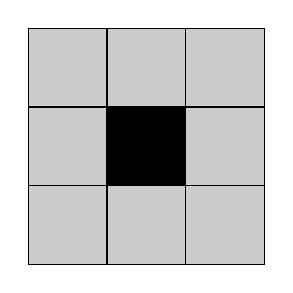
\begin{tikzpicture}%
	\tikzstyle{cell}=[rectangle, draw=black, minimum size=1cm];
	\node[fill=black] at (0, 0) [cell] {};
	\node[fill=black!20] at (1, 1) [cell] {};
	\node[fill=black!20] at (1, -1) [cell] {};
	\node[fill=black!20] at (-1, 1) [cell] {};
	\node[fill=black!20] at (-1, -1) [cell] {};
	\node[fill=black!20] at (0, 1) [cell] {};
	\node[fill=black!20] at (0, -1) [cell] {};
	\node[fill=black!20] at (-1, 0) [cell] {};
	\node[fill=black!20] at (1, 0) [cell] {};
	\end{tikzpicture}
\end{document}
